%!TEX root = ../neo4j.tex

\section{Storage Structure}

\subsection{Graph representation of the Data}
The simple sample graph displayed in figure \ref{fig1} shows a subgraph of the Neo4j example.
This human readable representation is now used to explain how Neo4j stores this graph. \nocite{storage1} \nocite{storage2}

\begin{figure}
	\centering
 	 	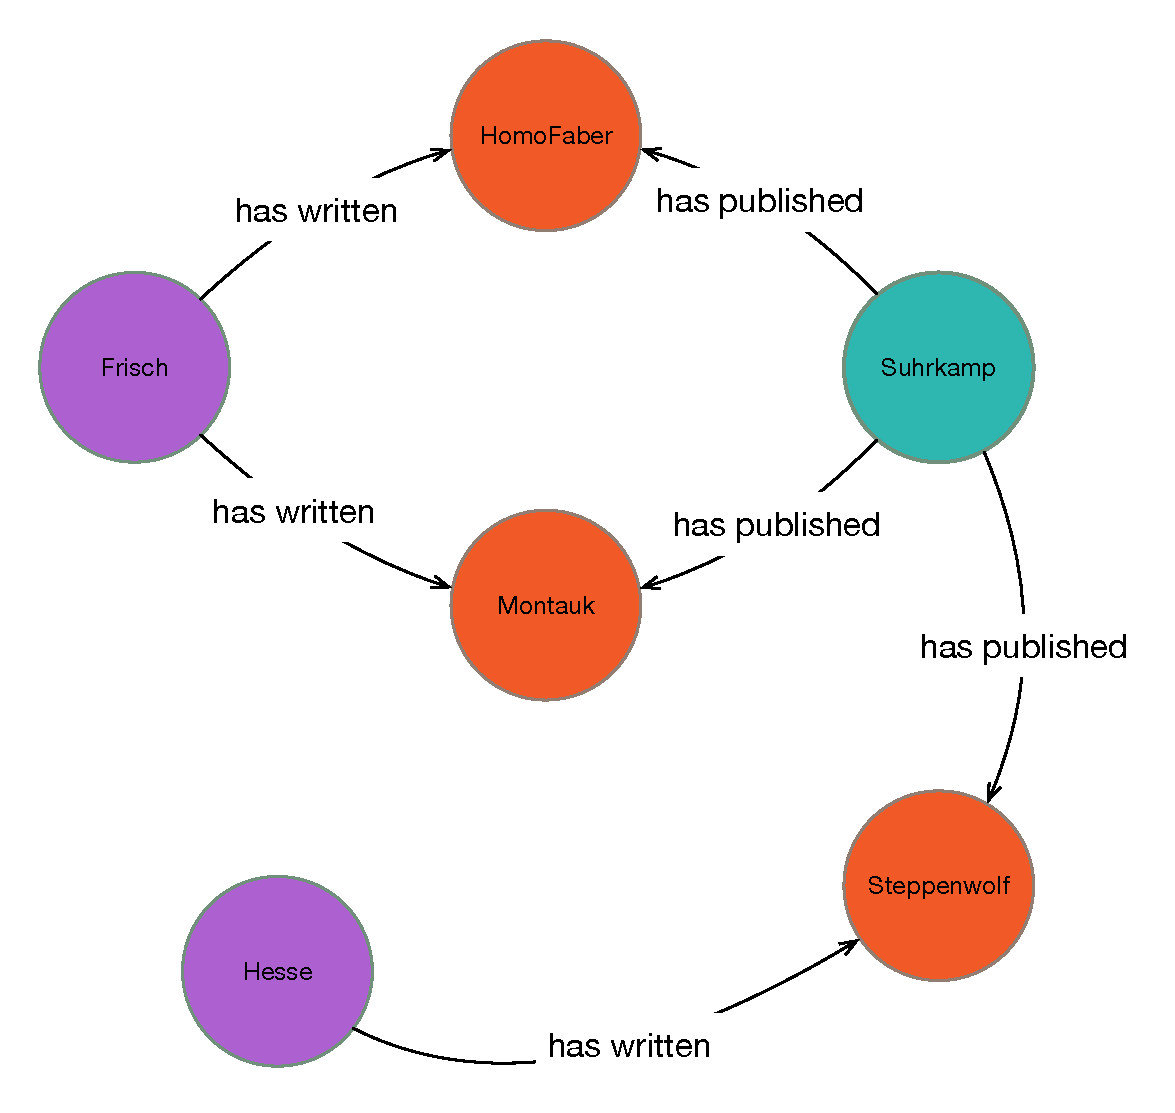
\includegraphics[width=0.9\textwidth]{images/theGraph.eps}
	\caption{Simple sample Graph}
	\label{fig1}
\end{figure}

\subsection{Property Records}
As a first step we take a look at the data stored in this graph. In Neo4j it is possible to store properties for every node and relationship (labels are ignored at the moment). To store the nodes and relationships itself in fixed size records (for faster access etc.) linked lists are used.
In figure \ref{fig2} the property records are displayed.

Every node and every relationship references its first property record. The property records themselves can be seen as a double linked list with a key - value store. In figure \ref{fig8} the representation on byte-level is shown. Node, relationship and property records are storing pointer to the next property in the last 4 bytes (one integer in Java). Bytes 18 to 21 of property record are containing a pointer to the previous record.


\begin{figure}
	\centering
 	 	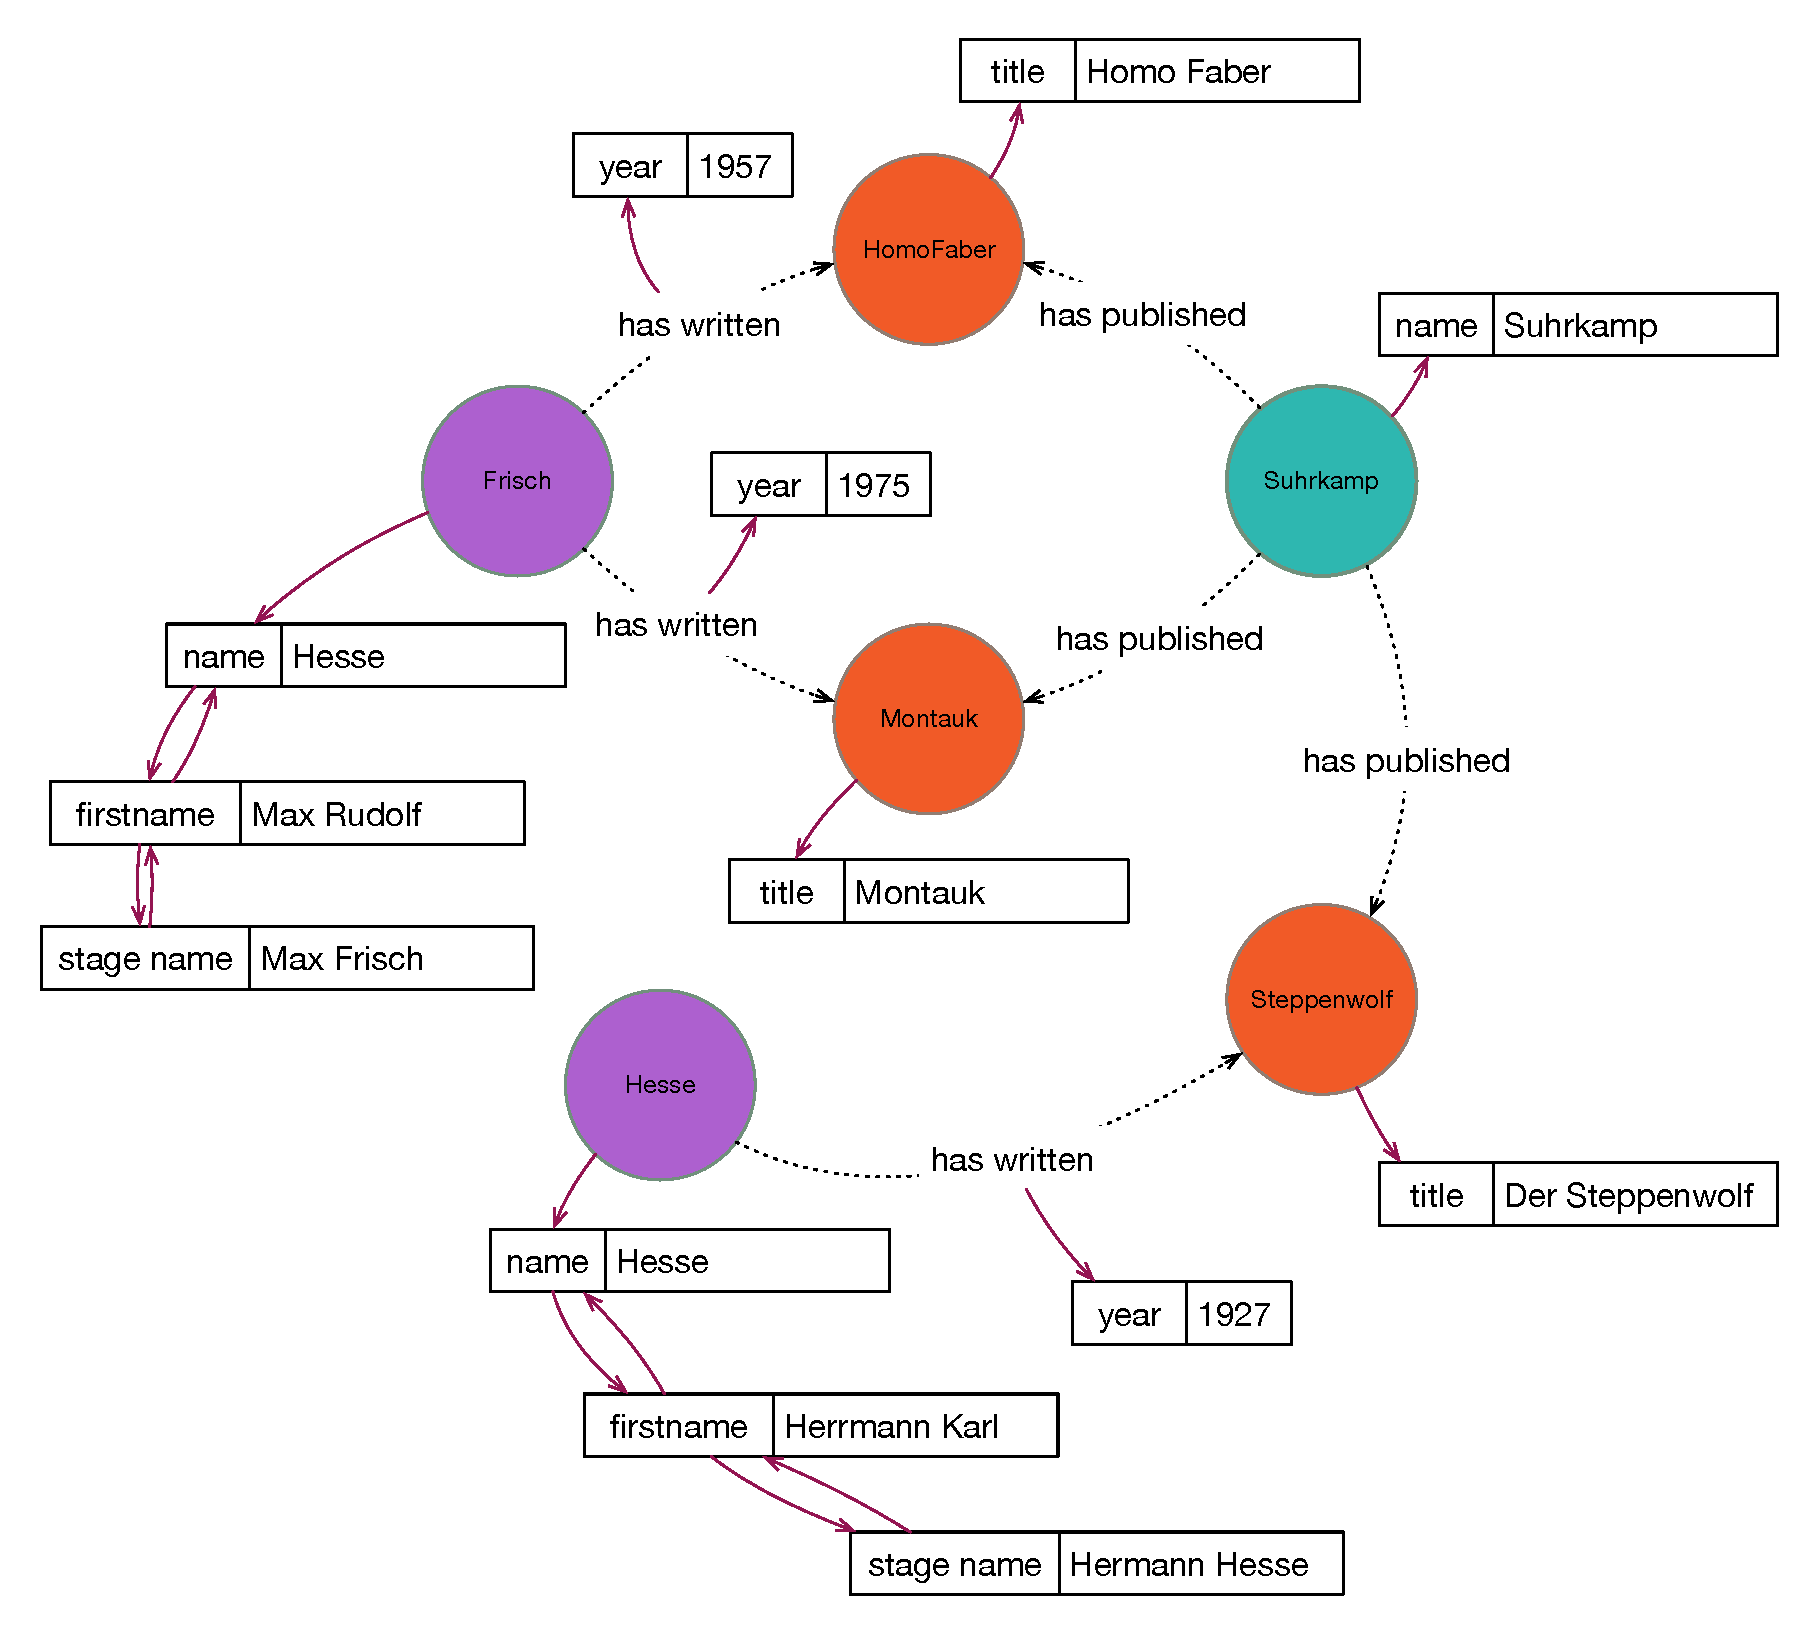
\includegraphics[width=0.9\textwidth]{images/nextProperty.eps}
	\caption{Property Records}
	\label{fig2}
\end{figure}

\subsection{Node Records}
The nodes itself as well as relationships are stored in fixed size records. However a node needs to know all relationships it is involved in. Therefor again a linked list is used. Every node references its first relationship shown in figure \ref{fig3} and in figure \ref{fig8} the deep blue marked bytes.
Now the complete node recored was covered and before we are focusing on the double linked relationship lists the relationship record is explained.

\begin{figure}[h]
	\centering
 	 	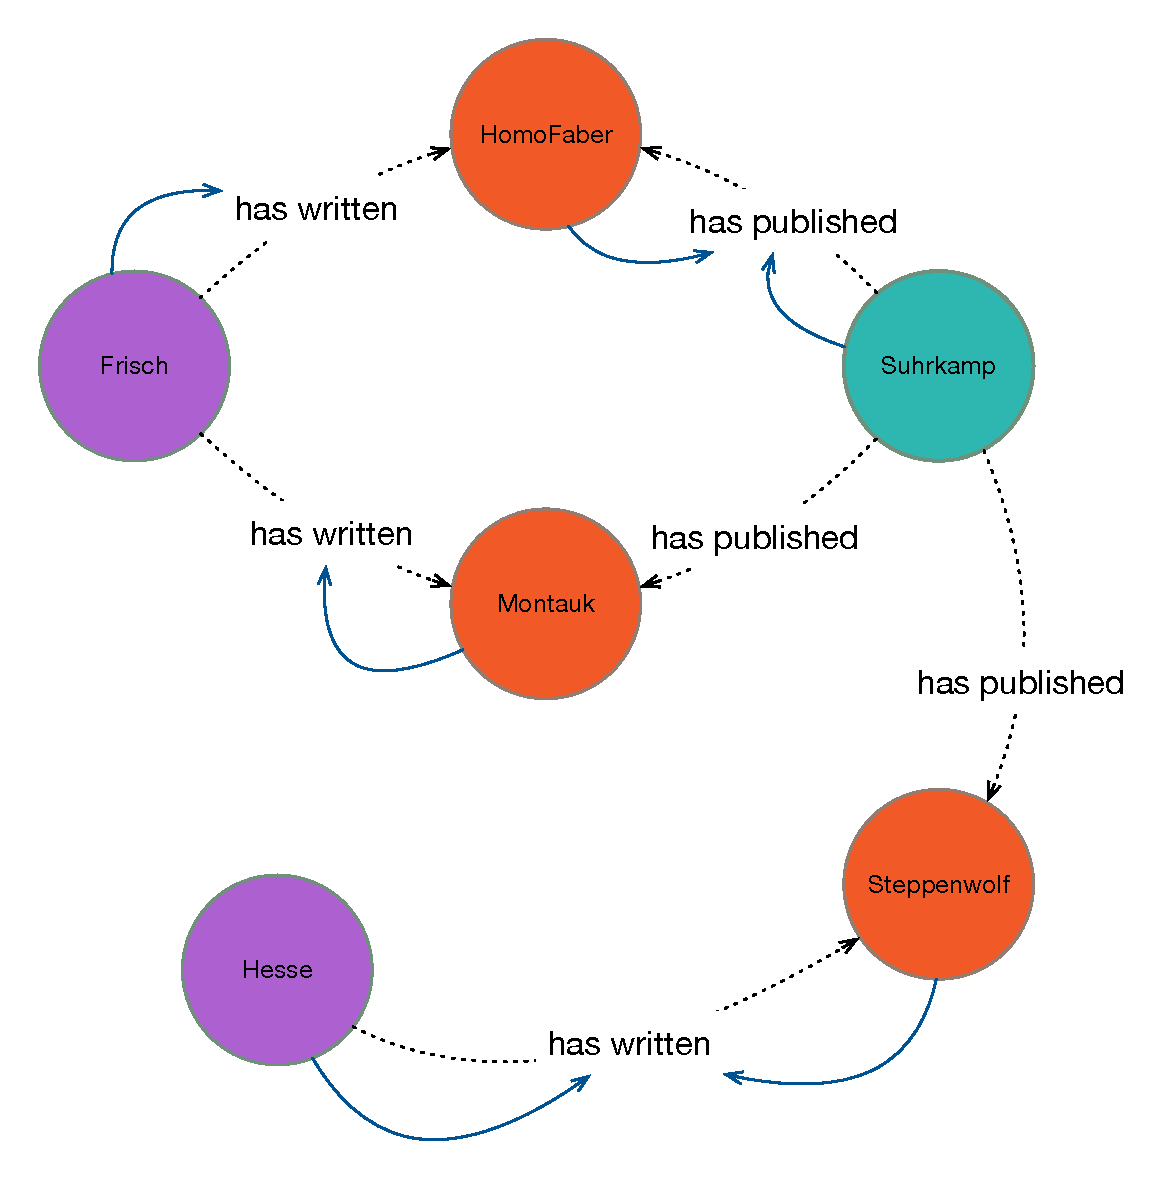
\includegraphics[width=0.9\textwidth]{images/nextRelationship.eps}
	\caption{First Relationship}
	\label{fig3}
\end{figure}

\subsection{Relationship Records}
As could have been observed above the node record only stores a pointer to a property and a relationship but not the first adjacent. Therefore we change our perspective to the graph and are focusing on relationships.
Instead of nodes referencing adjacent nodes we have nodes referencing the first relationship which references the start-node and the end-node of the relationship (Grey filled bytes in figure \ref{fig8}). This results in the abstract graph shown in figure \ref{fig4}.

The relationship type (Blue in figure \ref{fig4}) references a relationship type which again references a string (with the name) in the dynamic store. (This avoids redundancy in storage - the cache works in a different way.) 

The four green integers of the relationship record (figure \ref{fig8}) are used to realize the mentioned double linked relationship lists.
\begin{figure}
	\centering
 	 	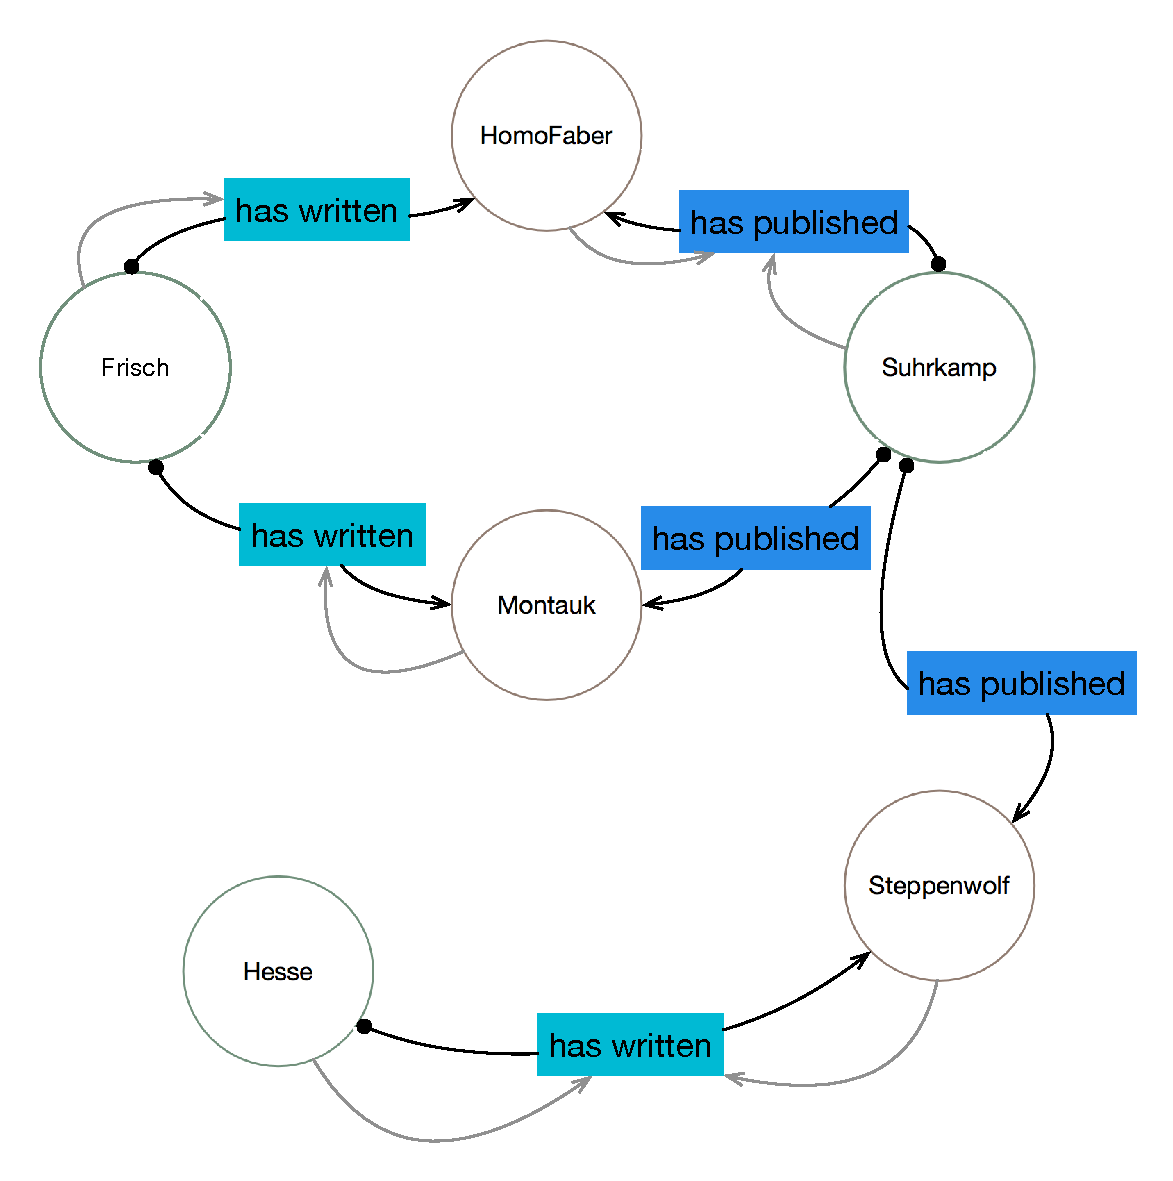
\includegraphics[width=0.9\textwidth]{images/startEnd.eps}
	\caption{Start Node - End Node}
	\label{fig4}
\end{figure}

Since every relationship is involved into two double linked lists (the one of the start-node and the one of the end-node) four pointers need to be stored.
In figure \ref{fig4}. They are shown as:

\begin{itemize}
	\item \textbf{SP} Start-Node Previous Relationship
	\item \textbf{EP} End-Node Previous Relationship
	\item \textbf{SN} Start-Node Next Relationship
	\item \textbf{EN} End-Node Next Relationship
\end{itemize}

In figure \ref{fig5} only the SP is set. In the following list some pointers are explained:
\begin{itemize}
	\item 'Frisch - has written - HomoFaber' has no pevious relationship since Frisch references it as its first relationship.
	\item 'Frisch - has written - Montauk' has 'Frisch - has written - HomoFaber' as previous relationship.
	\item 'Suhrkamp - has published - Steppenwolf' has 'Suhrkamp - has published - Montauk' which has  'Suhrkamp - has published - HomoFaver' which has no previous relationship.
	\item \dots
\end{itemize}

\begin{figure}
	\centering
 	 	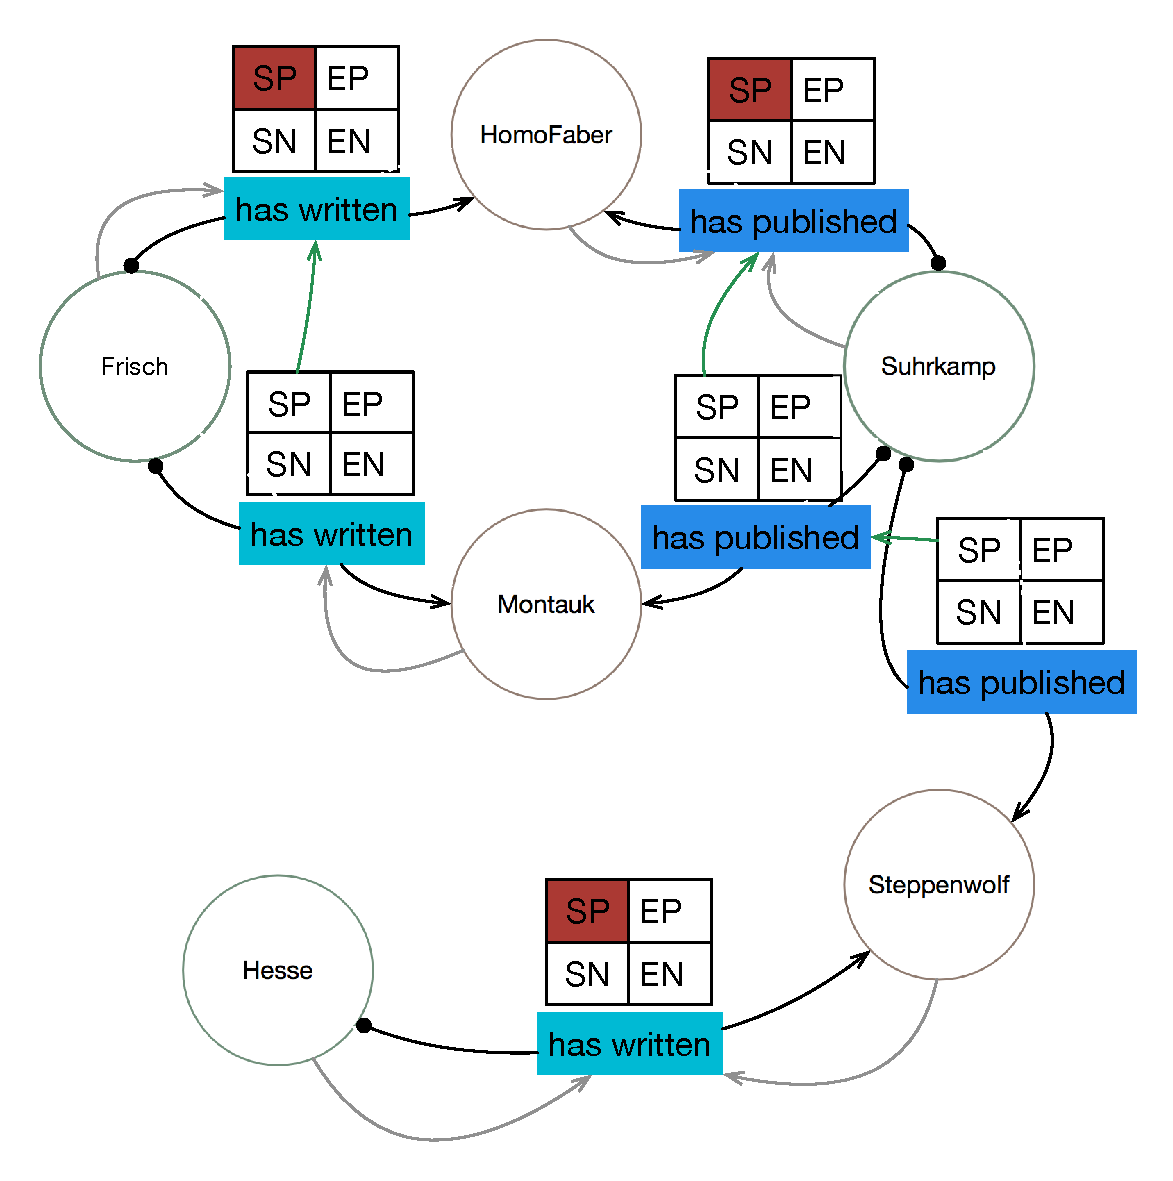
\includegraphics[width=0.9\textwidth]{images/StartNodePrevRel.eps}
	\caption{Start Node Previous Relationship}
	\label{fig5}
\end{figure}

In figure \ref{fig6} the links for the end-node previous relationship are added analogue to start-node previous relationship.

\begin{figure}
	\centering
 	 	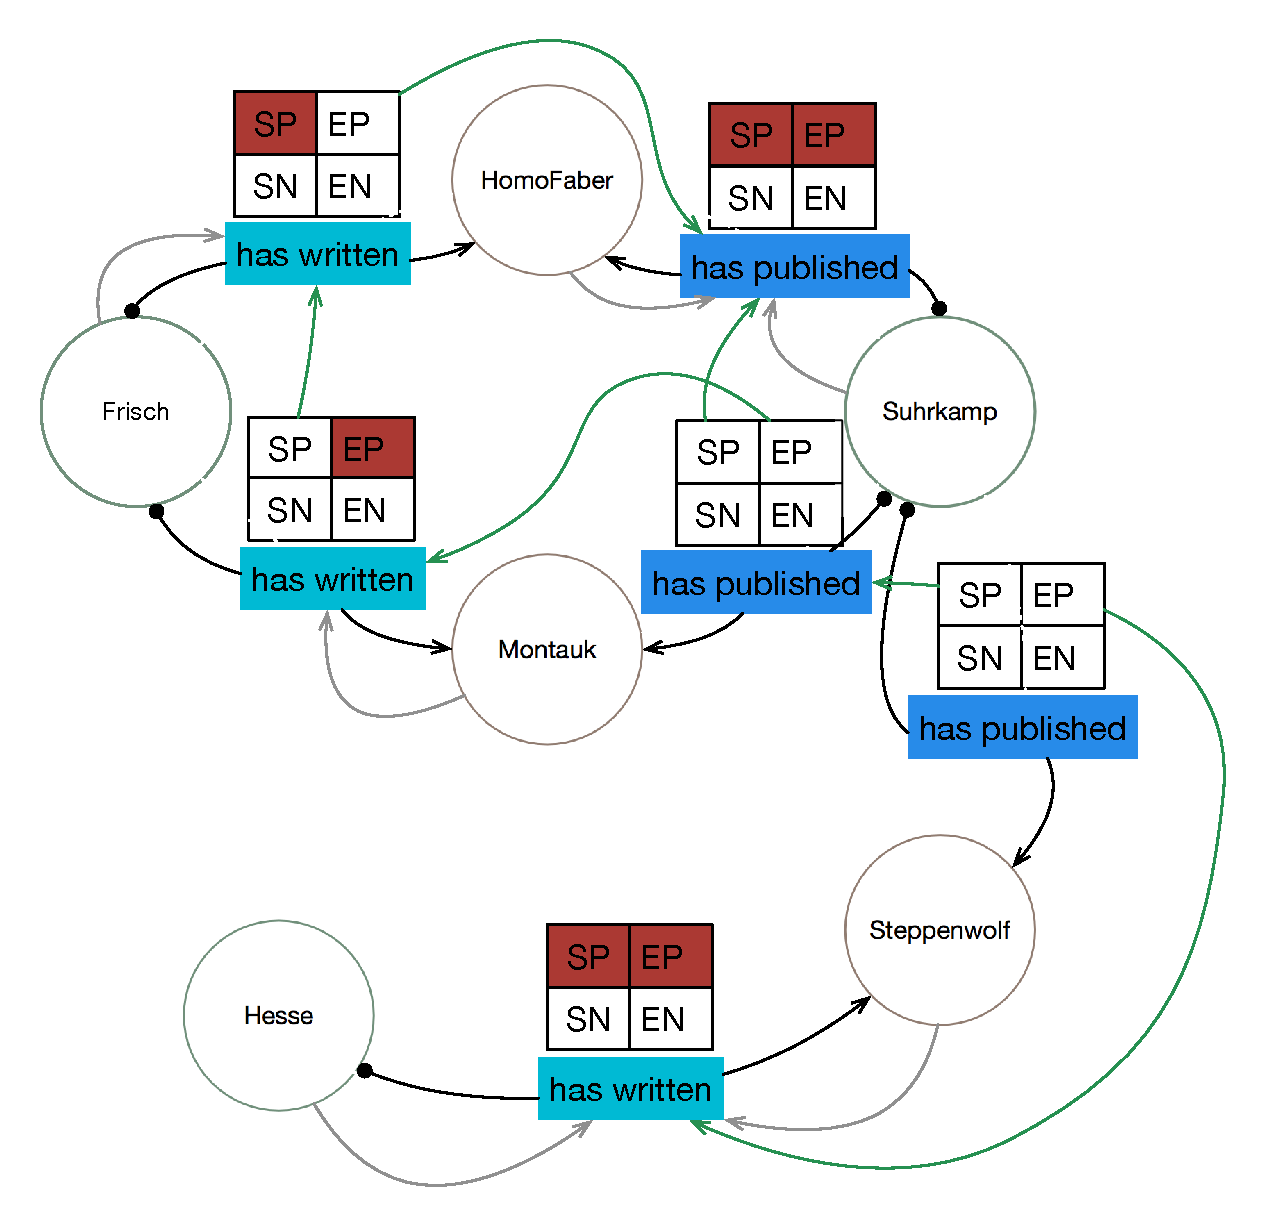
\includegraphics[width=0.9\textwidth]{images/EndNodePrevRel.eps}
	\caption{End Node Previous Relationship}
	\label{fig6}
\end{figure}

Now in figure \ref{fig7} all double linked lists are complete. This is how the graph displayed in figure \ref{fig1} would be stored. 

\begin{figure}
	\centering
 	 	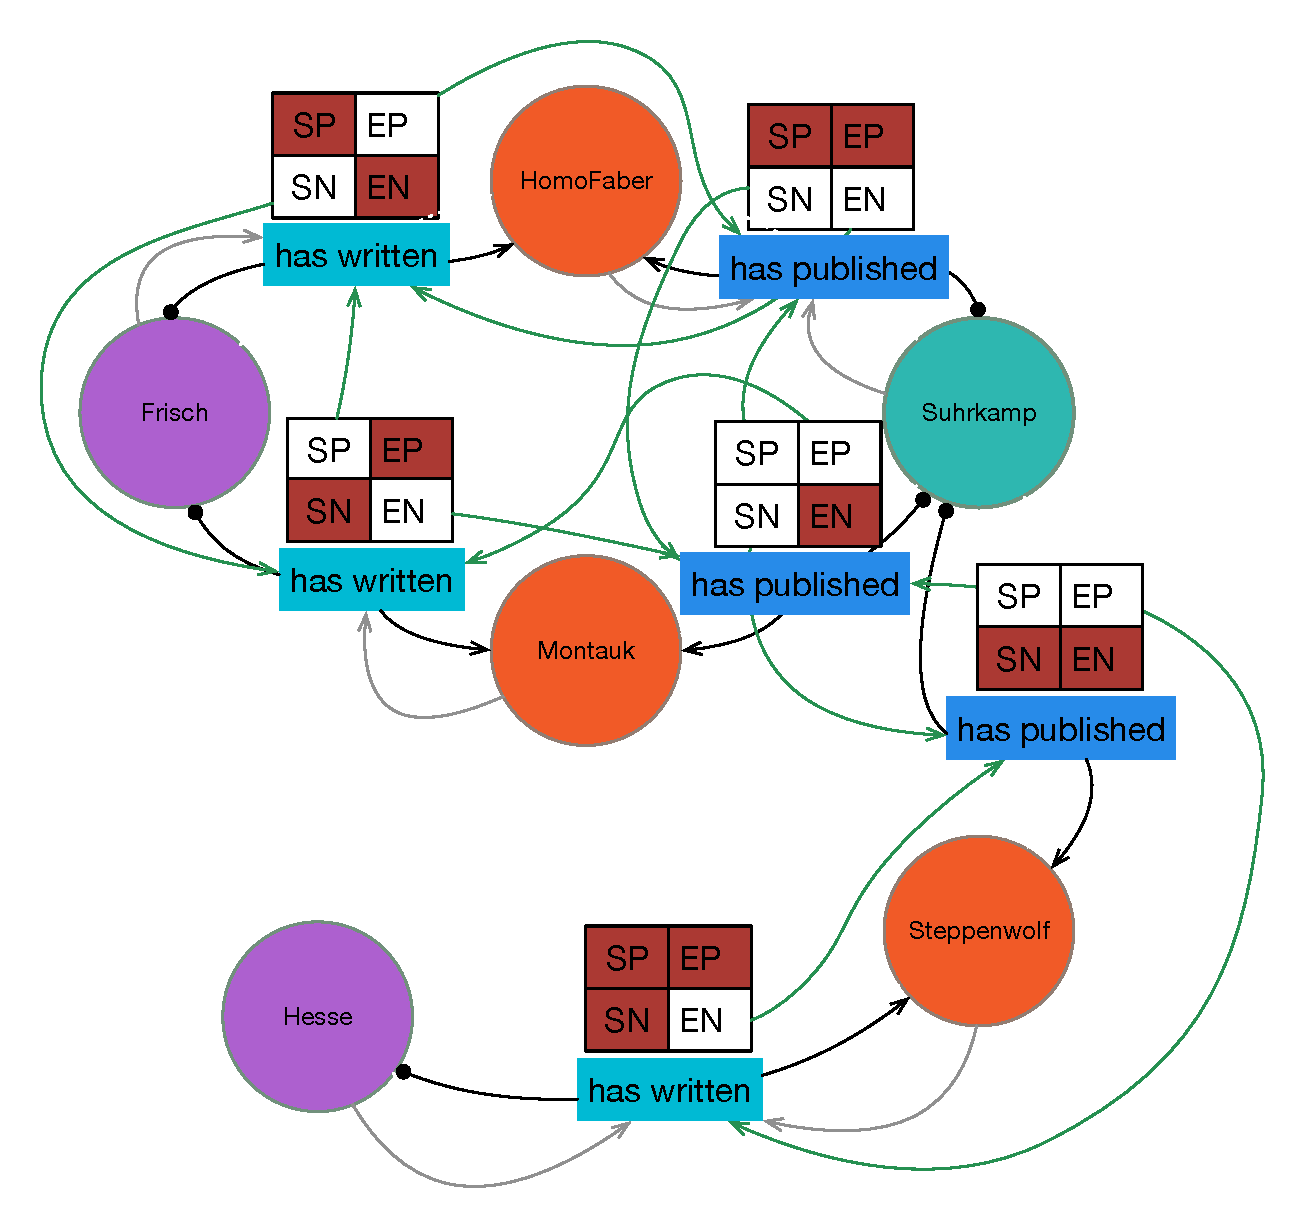
\includegraphics[width=0.9\textwidth]{images/complete.eps}
	\caption{All Pointers Displyed}
	\label{fig7}
\end{figure}

\begin{figure}
	\centering
 	 	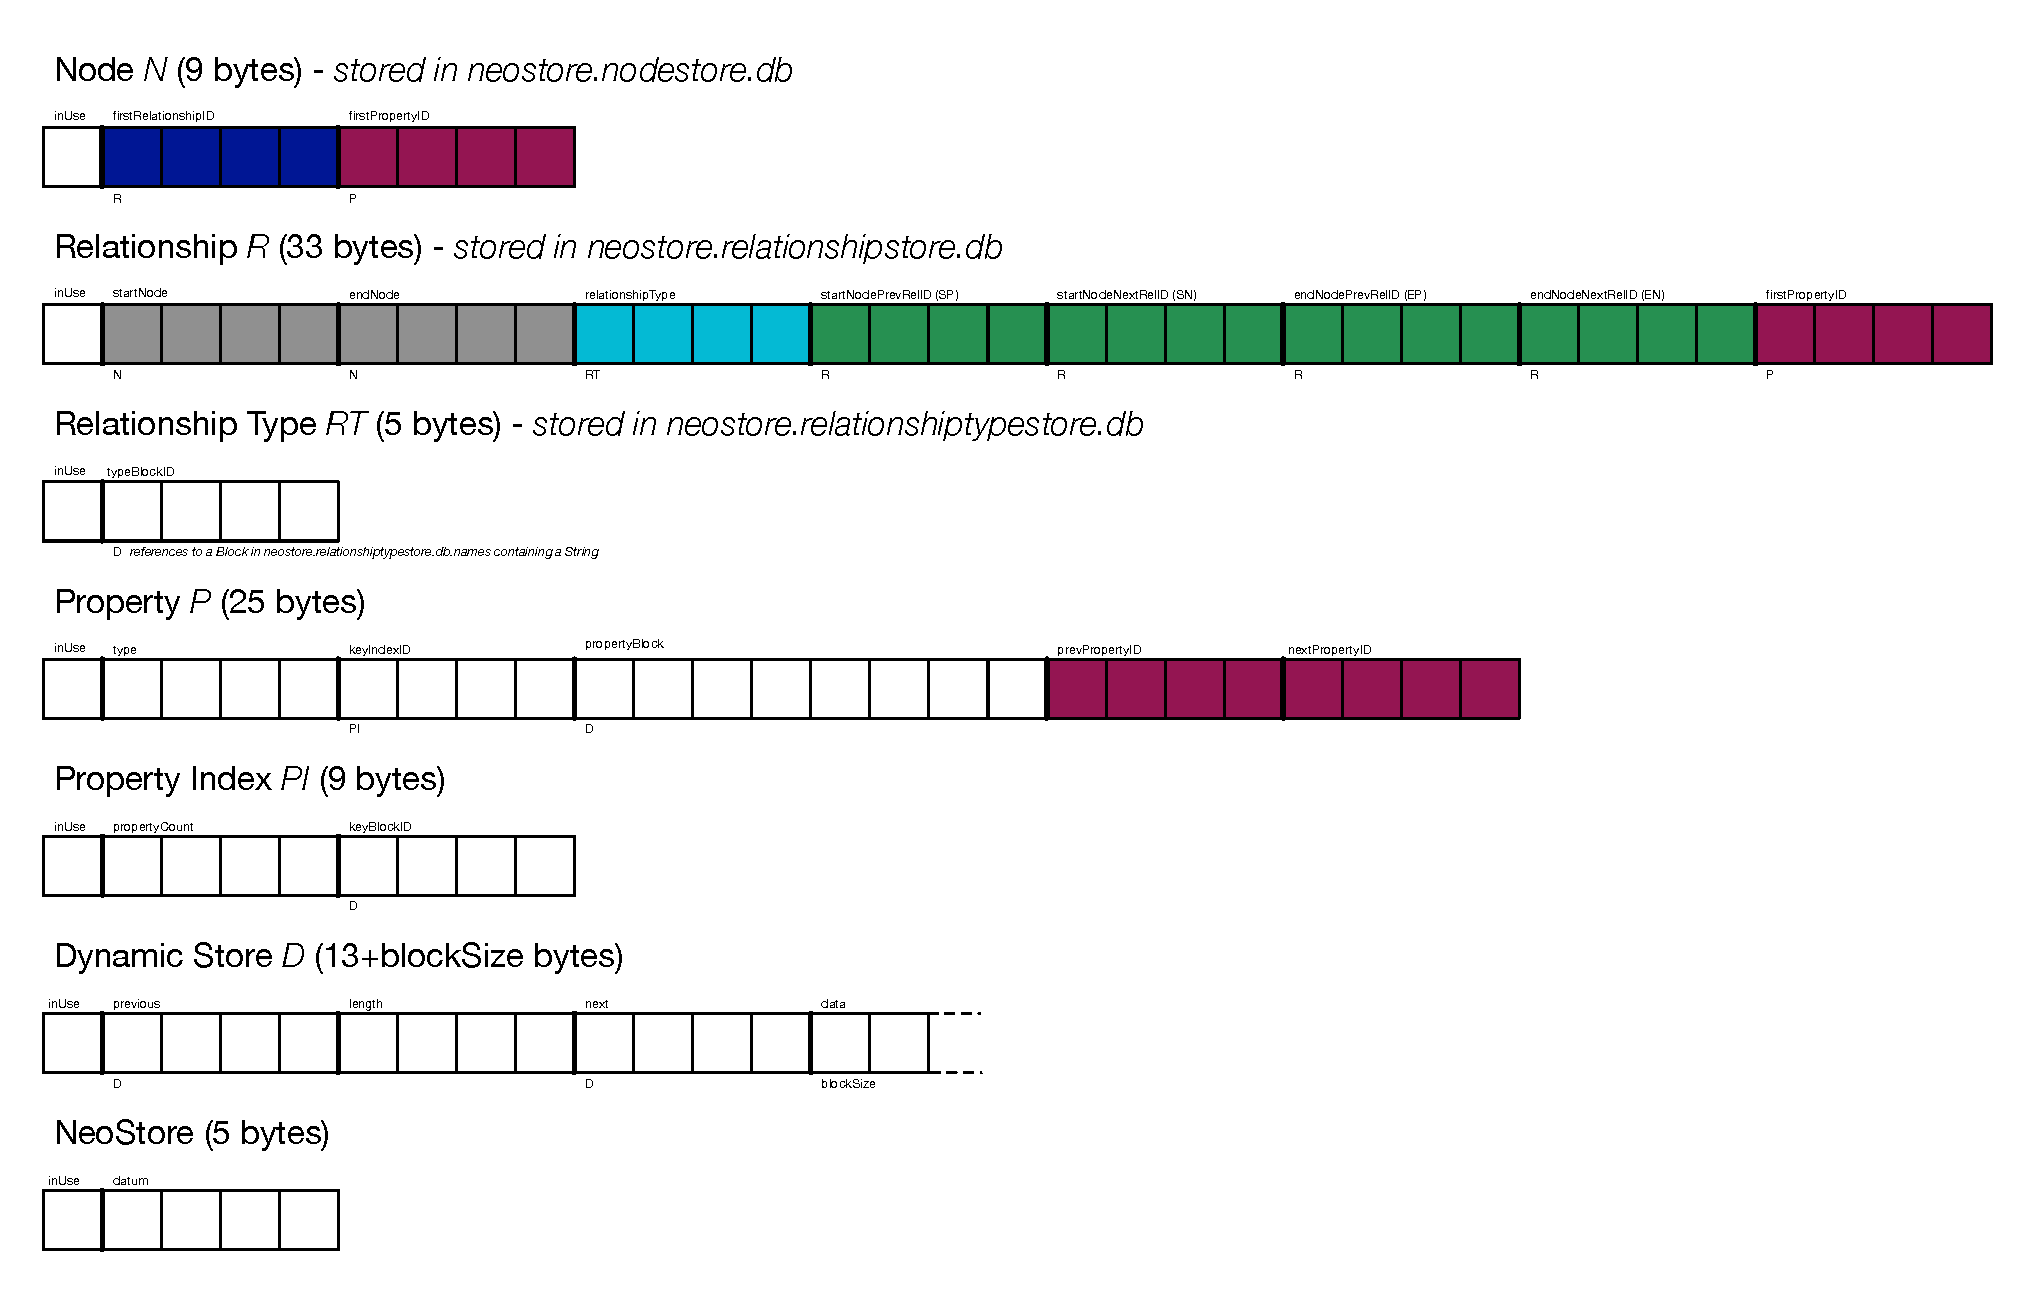
\includegraphics[width=1.2\textwidth, angle=90]{images/NeoBytes.eps}
	\caption{NeoBytes}
	\label{fig8}
\end{figure}
